\documentclass{article}
\usepackage[utf8]{inputenc}
\usepackage{listings}
\usepackage{tabularx}
\usepackage{url}
\usepackage{pgfplots}
\pgfplotsset{compat=1.14}

\title{CS3910 Computational Intelligence:\\Cutting Stock Problem (Coursework 1)}
\author{Scott Street\\{\small 159027651}}
\date{December 2017}

\begin{document}
\maketitle

\section{Introduction}

  The Cutting Stock Problem (CSP) is a combinatorial optimisation problem, in which we are given a set of stock lengths with associated costs, a set of order lengths with associated quantities, and must cut the ordered lengths from the given stock, while attempting to minimise the cost of materials.

  For this coursework, implementations have been written in the Go programming language, for its high efficiency and concurrency features (not used in this version of the implementation, but potentially in future versions).

\section{Problem Representation}

  The problem instance is represented as a simple \lstinline{struct} containing the provided stock lengths, stock costs, order lengths, and order quantities. Each of these is contained within a \lstinline{slice} (variable length array).

  Solutions to the a problem instance are implemented as a 2D \lstinline{slice} of \lstinline{int}s, where the top level represents the available stock lengths, and the individual elements represent ordered lengths. It is not necessary to keep track of how many stock lengths of each type have been used, as it is not required for the running of either of the implemented algorithms, and can be calculated from this representation when needed.

\section{Algorithm Implementations}

  The Artificial Immune System (AIS) and Ant Colony Optimisation (ACO) algorithms were selected for use due to the combinatorial nature of the CSP. Both algorithms are well suited to such problems, whereas it may be the case that algorithms which are typically used to solve, for example, continuous problems are not as easily translated for use in this situation.

  \subsection{Artificial Immune System}

  The AIS immune system approach is inspired by the human immune system. Specifically, the Clonal Selection algorithm (CLONALG) applies the theory that white blood cells improve their ability to counter alien cells over time, as they are exposed to them. In the case of the CSP, the algorithm improves its ability to produce more optimal solutions as it discovers them.

  It does this through a method of cloning, mutation, and selection. From an initial population of a specified size, a clone pool is created by "copying" the existing population x-number of times (a parameter to the algorithm). The pool is then mutated through some process. In this implementation, the mutation function selects a random neighbour from the solution's two-opt neighbourhood.

  The mutated pool is then added back to the main population, at which point the selection process takes place. This decides which of the population are kept for the next generation, up to a defined number. A simple greedy method of selection has been used in this instance.

  Finally, a form of metadynamics are performed on the population - the lowest n-number of the populus are replaced by random solutions. Additionally, the "age" of each solution in the population is incremented, until reaching the defined maximum age, at which point is it removed from the population. Both of these methods prevent the algorithm from reaching "stale" solutions, or local minima. By ensuring this degree of randomness, we are guaranteed to eventually reach the optimal solution for a given problem instance.

  \subsection{Ant Colony Optimisation}

    Reference that paper\cite{acoforcsp} at some point.

\section{Comparison of Algorithms}

  Todo.

  Avg over 40

  Problem 2
  CLONALG(instance, time, 20, 10, 5, 100)
  1: 5175
  5: 5044
  10: 4926
  20: 4804
  40: 4660
  80: 4542

  ACO (probably invalid)
  1: 5533
  5: 5446
  10: 5428
  20: 5362
  40: 5278

  \newcolumntype{R}{>{\raggedleft\arraybackslash}X}%
  \noindent\begin{tabularx}{\textwidth}{ |l|R|R|R|R|R|R| }
    \hline
    Algorithm & 1 run & 5 runs & 10 runs & 20 runs & 40 runs & 80 runs \\
    \hline
    CLONALG   & 5175  & 5044   & 4926    & 4804    & 4660    & 4542    \\
    \hline
    ACO       & 5533  & 5446   & 5428    & 5362    & 5278    & -       \\
    \hline
  \end{tabularx}

  \bigskip

  \begin{center}
    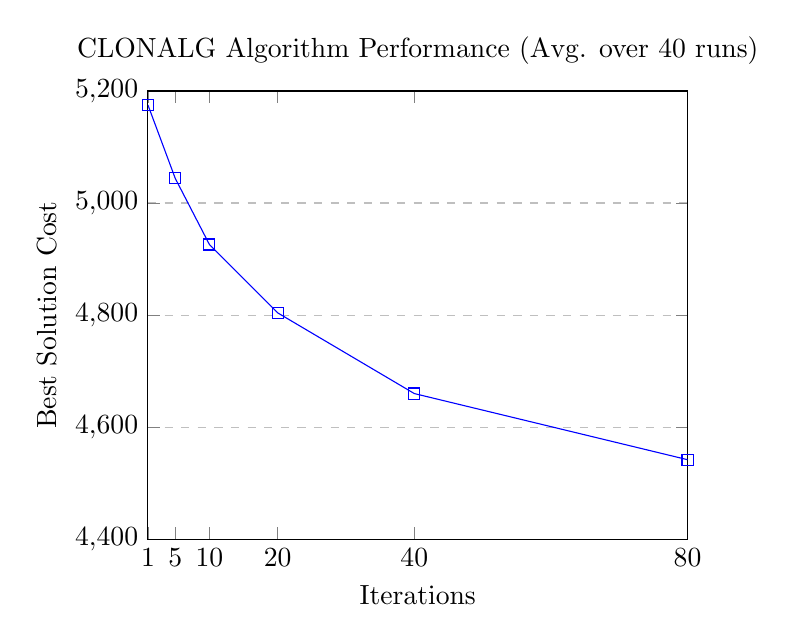
\begin{tikzpicture}
      \begin{axis}[
          title={CLONALG Algorithm Performance (Avg. over 40 runs)},
          xlabel={Iterations},
          ylabel={Best Solution Cost},
          xmin=1, xmax=80,
          ymin=4400, ymax=5200,
          xtick={1,5,10,20,40,80},
          ytick={4400,4600,4800,5000,5200},
          legend pos=north west,
          ymajorgrids=true,
          grid style=dashed,
      ]

        \addplot[
            color=blue,
            mark=square,
            ]
            coordinates {
            (1,5175)(5,5044)(10,4926)(20,4804)(40,4660)(80,4542)
            };

      \end{axis}
    \end{tikzpicture}
  \end{center}

  \bigskip

\bibliography{report}
\bibliographystyle{plain}

\end{document}
